% Chapter: aitranss module

%%%%%%%%%%%%%%%%%%%%%%%%%%%%%%%%%%%%%%%%%%%%%%%%%%%%%%%%%%%%%%%%%%%%%%%
\section{Source code and supporting materials} 
\label{sec:aitranss:source}

The source code and supporting material of the \textsc{aitranss}-module
for the FHI-aims package is placed in the subdirectory \verb,aitranss/,.
This directory contains subdirectories:

\begin{itemize}
 \item \verb,source/, : with the Fortran90 code and the example
   \verb,Makefile, ; 
 \item \verb,tcontrol.script/, : contains a script
 \verb,tcontrol.aims.x,,
   which is served to prepare a mandatory input file \verb,tcontrol,
   for the transport-type calculation ;
 \item \verb,electrodes.library/, : contains a library of representative
   gold (Au) clusters
   (xyz-files) which should be linked, via anchoring groups, to your
   molecular system to create an ``extended molecule'': its electronic
   structure (Kohn-Sham molecular orbitals and energies) is a prerequisite
   to compute transport characteristics ;
 \item \verb,examples/, : contains examples, with input and output
   files of the FHI-aims and \textsc{aitranss}; \verb,README, files
   found in this subdirectory contain also short guidelines on how an
   input for a particular transport calculation has been created.
\end{itemize}

\section[Compiling the \textsc{aitranss} module]%
{Compiling the {\large AITRANSS} module}
\label{sec:aitranss:compiling}

Please, use a template of the \verb,Makefile, found in the directory
\verb,source/,, and adjust variables referring to compiler (\verb,FC,
and \verb,LD,), compiler's options (\verb,FLAGS,) and a path to libraries
(\verb,LIBS,) at your computer system.  A mandatory prerequisite to build 
the code is a Fortran 90/95 capable compiler and a compiled version of 
{\small{LAPACK}} and {\small{BLAS}} (for example, Intel's {\small{MKL}}). 
A~binary (\verb,aitranss.x,) built by the \verb,Makefile, will go to the 
\verb,bin/, directory of the FHI-aims.

In contrast to FHI-aims, the current release of \textsc{aitranss}
is not yet based on MPI. However, you are encouraged to use a fortran
compiler option(s), aka \verb,"-openmp", and \verb,"-O2", for Intel's
\verb,ifort,,\ to enable the auto-parallelizer to build a multithreaded
code based on OpenMP directives.

According to our experience, a generated code can be safely executed in
parallel within a single compute node with multiple processors, and with
a significant gain in computation time.

We advise you as well to copy a script \verb,tcontrol.aims.x, found
in the directory \linebreak \verb,tcontrol.script/, to the directory
\verb,bin/, of the FHI-aims installation, and to make files in that
directory accessible for the execution from a command line by adjusting
your shell variable \verb,PATH,.

\clearpage

%%%%%%%%%%%%%%%%%%%%%%%%%%%%%%%%%%%%%%%%%%%%%%%%%%%%%%%%%%%%%%
\section{How to set-up and run transport calculations}
%%%%%%%%%%%%%%%%%%%%%%%%%%%%%%%%%%%%%%%%%%%%%%%%%%%%%%%%%%%%%%
\label{sec:aitranss:howto}

\subsection{FHI-aims run: input and output} 
\label{subsec:fhiaims}

Having your molecule "at hands", use your favorite modeling and
visualization tools/\-software, and prepare an extended structure
by linking the molecule via anchoring groups to two atomic clusters,
representing parts of macroscopic \textit{source} and \textit{drain}
electrodes.  Consult the \verb,electrodes.library/, directory, and
use predefined Au clusters found there.  A typical example of an
``extended molecule'', which you are requested to build, is shown in
Fig.~\ref{fig:extended_molecule}.

Include a line

\noindent
\phantom{xxx}\keyword{output}\ \subkeyword{output}{aitranss}
%\begin{verbatim}
%   output aitranss
%\end{verbatim}

\noindent
into your \verb,control.in, file. Furthermore, following settings are
recommended for the self-consistent DFT calculation:

\begin{verbatim}
  occupation_type    gaussian 0.1
  mixer              pulay
    n_max_pulay        10
    charge_mix_param   0.2

  sc_accuracy_rho    1E-4
  sc_accuracy_eev    1E-2
  sc_accuracy_etot   1E-6

  relativistic zora scalar 1.0e-10
\end{verbatim}

Invoke FHI-aims exploiting a cluster type (non-periodic)
calculation. After the FHI-aims run is finished, you'll find in your
directory three ASCII files: \verb,basis-indices.out,, \verb,omat.aims,
and \verb,mos.aims,. These files contain: some limited information on
basis functions; overlap integrals; and data on Kohn-Sham molecular
orbitals \& energies of the ``extended molecule'', respectively. If
spin channels of your system are not identical, \verb,mos.aims,
will be substituted by two other files called \verb,alpha.aims, and
\verb,beta.aims,.

\subsection[What to be aware of before running \textsc{aitranss} module]%
{What to be aware of before running {\normalsize AITRANSS} module} 
\label{subsec:aitranss:whattobeaware}

The \textsc{aitranss} module should be run from the same directory,
where output files of FHI-aims are placed.  A file \verb,geometry.in,
is mandatory and should also be there.

A file \verb,control.in, is not used. Instead, another mandatory file for
the transport calculation is \verb,tcontrol,.  Please, \textit{always} use
a script \verb,tcontrol.aims.x, to create this file.  Executing a script
\verb,tcontrol.aims.x, without arguments outputs a help information:

\clearpage

\begin{verbatim}
[...]
--------------------------------------------------------------
"tcontrol.aims.x"   script creates a mandatory file "tcontrol"
                    which is required to run the "aitranss"
                    post-processing module after FHI-aims
--------------------------------------------------------------
USAGE: tcontrol.aims.x [ -option <argument> ] ...

where options & arguments are:

                       ! electrodes geometry:
 -lsurc <atom1>        three atoms which define an outermost
 -lsurx <atom2>        LEFT surface layer of the extended
 -lsury <atom3>        molecule

 -rsurc <atom4>        three atoms which define an outermost
 -rsurx <atom5>        RIGHT surface layer of the extended
 -rsury <atom6>        molecule

 -nlayers <number>     number of atomic layers coupled to 
                       reservoirs via a self-energy

                       ! energy window, in Hartree [H], to
                       ! output transmission function T(E) :
 -ener  <E1[H]>        initial energy point, E1
 -estep <dE[H]>        energy step, dE
 -eend  <E2[H]>        final energy point, E2

                       ! output :
 -outfile <file_name>  output file name for T(E) [default: TE.dat]

\end{verbatim}

When executed with options and arguments, a script \verb,tcontrol.aims.x,
checks for the \verb,geometry.in, file and other mandatory FHI-aims
output files (\verb,basis-indices.out,, \verb,omat.aims,, \verb,mos.aims,
or \verb,alpha.aims, \& \verb,beta.aims,) in your directory, reads from
these files information on a system size and the Hamiltonian $H$ and
overlap matrix dimension, and exports this information together with
your arguments to an ASCII file \verb,tcontrol,. Options and arguments
are used: (i) to provide information on the self-energy construction;
(ii) to introduce an energy window for the calculation of the transmission
function $T(E)$, and (iii) (optionally) to introduce an output file name
for $T(E)$.

\begin{figure} 
\centering
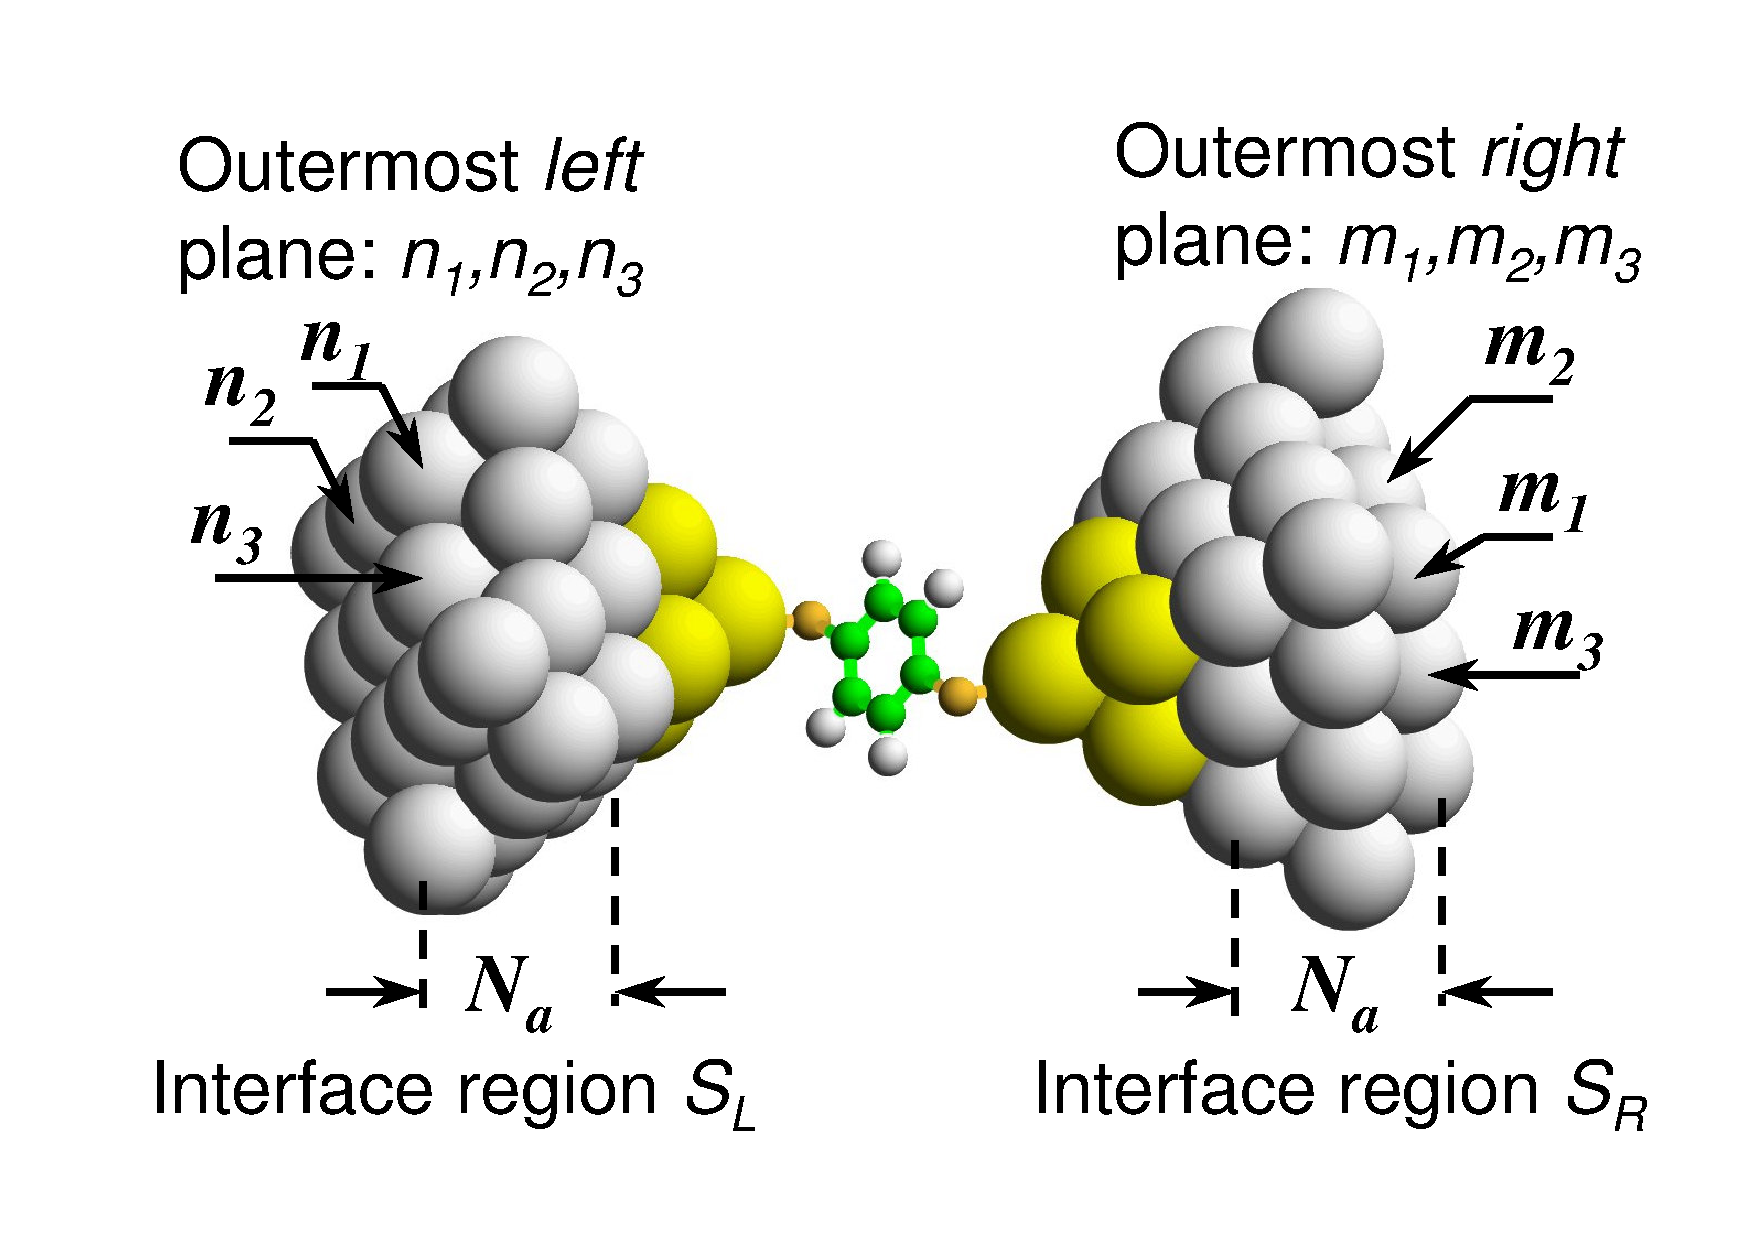
\includegraphics[width=0.6\textwidth]{fig_extended_molecule.pdf}
\caption{% 
\label{fig:extended_molecule} A schematic view of the
``extended molecule''.  The shaded regions are interfaces to the two
reservoirs. Within the interface regions absorbing boundary conditions
are active and the self-energy $\Sigma$ is introduced. A user defines
interface regions by specifying the outermost \textit{left} and
\textit{right} atomic planes (introducing indices of three different atoms
that form a triangle, $n_1,n_2,n_3$, and $m_1,m_2,m_3$, respectively)
and the amount of atomic layers, $N_a$.  } 
\end{figure}

\emph{Comment on the self-energy}. When an ``extended molecule''
is contacted to macroscopic reservoirs, a propagation of an electron
with energy $E$ within a subspace limited by the ``extended molecule''
is described by the Green's function: $ G^{-1}(E) = E - H - \Sigma(E)
$, where a self-energy $\Sigma(E)$ accounts for the interaction
between a finite system and macroscopic reservoirs.  As argued in
Refs.~\cite{Arnold2007,Evers2006}, if atomic clusters introduced to model parts
of metallic electrodes are large enough, the reservoirs can be modeled
by absorbing boundary conditions which become active at the interface
regions ${\cal S}_L$ and ${\cal S}_R$ (labeled by a gray color in
Fig.~\ref{fig:extended_molecule}) where the ``extended molecule'' is
coupled to reservoirs. Within this model, the self-energy is approximated
by an energy-independent, diagonal matrix, 
\[
 \Sigma^{\mu\mu'}_{nn'} \approx - i \eta_n \delta_{nn'}\delta_{\mu\mu'},
\] 
where indices $n$ and $n'$ label atoms, and $\mu$ and $\mu'$ label
corresponding internal degrees of freedom (i.e., atom-centered basis
functions). Here absorption rates $\eta_n$ are allowed to have non-zero
weights only within the interface regions ${\cal S}_L$ and ${\cal S}_R$.
A user defines interface regions by specifying the outermost \textit{left}
and \textit{right} atomic planes (introducing indices of three different
atoms forming a triangle, $n_1,n_2,n_3$, and $m_1,m_2,m_3$, respectively)
and the amount of atomic layers, $N_a$.  
%{\bf AB: Is the number of layers for left and right hand side the same?}

\subsection{% 
How to create a mandatory file \texttt{tcontrol}}
\label{subsec:aitranss:tcontrol}

To create a \verb,tcontrol, file, a \verb,tcontrol.aims.x, script should
be launched with the following options and arguments:

\verb,tcontrol.aims.x, 
\verb,-lsurc, $n_1$ 
\verb,-lsurx, $n_2$
\verb,-lsury, $n_3$ 
\verb,-rsurc, $m_1$ 
\verb,-rsurx, $m_2$ 
\verb,-rsury, $m_3$ 
\verb,-nlayers, $N_a$ 
\verb,-ener, $E_1$ 
\verb,-estep, $dE$
\verb,-eend, $E_2$

\begin{itemize}

\item where integer numbers $n_1$, $n_2$, $n_3$ are indices of three
 different atoms fixing the outermost \textit{left} atomic plane of the
 ``extended molecule'' (see Fig.~\ref{fig:extended_molecule}); atoms are
 numbered according to their appearance in file \verb,geometry.in, ;

\item integer numbers $m_1$, $m_2$, $m_3$ are indices of three different
 atoms fixing the outermost \textit{right} atomic plane of the ``extended 
 molecule'' (see Fig.~~\ref{fig:extended_molecule});

\item an integer $N_a$ indicates the number of atomic layers
 defining the interface regions ${\cal S}_L$ and ${\cal S}_R$  (see
 Fig.~\ref{fig:extended_molecule}); users are strongly advised to take Au
 clusters of similar size from the directory \verb,electrodes.library/, and
 use a parameter $N_a$ suggested in the header of a library file.  Using Au
 clusters of similar size insures that $N_a$ can be consistently chosen to
 be the same for both \textit{left} and \textit{right} interface regions;

\item real numbers $E_1$, $E_2$ and a positive real number $dE$ define the
 energy window $[E_1,E_2]$ and energy step $dE$ to calculate transmission
 function $T(E)$;

\item optionally, you can launch the script with "\verb,-output,
 \textit{filename}" where \textit{filename} is a string, specifying a
 name of the output file for $T(E)$.  
\end{itemize}
 
An example of the transport calculation set-up for the
Au-benzene-dithiol-Au\ junction can be found in the directory
\texttt{examples/au-c6h6-au/}.  A script \texttt{tcontrol.aims.x} has
been executed there with the following options and arguments:

\begin{verbatim} 
tcontrol.aims.x -lsurc 34 -lsurx 30 -lsury 36 -rsurc 35 -rsurx 33
 -rsury 31 -nlayers 2 -ener -0.4000 -estep 0.0001 -eend 0.0000
\end{verbatim}

to create the following file \verb,tcontrol,:

\begin{verbatim}
#input data for the aitranss module
$aims_input on
$landauer on
$coord   file=geometry.in
$natoms  50
$basis   file=basis-indices.out
$read_omat file=omat.aims
$scfmo   file=mos.aims
$nsaos   2268
$ecp     on
$lsurc   34
$lsurx   30
$lsury   36
$rsurc   35
$rsurx   33
$rsury   31
$nlayers 2
$s1i     0.1d0
$s2i     0.05d0
$s3i     0.025d0
$ener   -0.4000
$estep   0.0001
$eend    0.0000
$output  file=TE.dat
$testing off
$end
\end{verbatim}

Detailed description of keywords in file  \verb,tcontrol, are given in
the paragraph~\ref{sec:aitranss:keywords}.

%%%%%%%%%%%%%%%%%%%%%%%%%%%%%%%%%%%%%%%%%%%%%%%%%%%%%%%%%%%%%
\subsection{% 
How to submit a transport calculation and its output} 
\label{subsec:aitranss:calc}
%%%%%%%%%%%%%%%%%%%%%%%%%%%%%%%%%%%%%%%%%%%%%%%%%%%%%%%%%%%%%

Assuming a binary file \verb,aitranss.x, is placed\ in the directory
\verb,bin/, of the FHI-aims installation\ which is referenced in your
shell variable \verb,PATH,, you can run the transport type calculation
from a command line, like

\verb,> aitranss.x | tee my.transport.calc.out,

or

\verb,> nohup aitranss.x > my.transport.calc.out &,

FHI-aims output files together with information provided from files
\verb,tcontrol, and \linebreak \verb,geometry.in, will be used by the
\textsc{aitranss} module to reconstruct a Kohn-Sham Hamiltonian ($H$) of the
``extended molecule'', to supplement $H$ with the self-energy $\Sigma$,
and to compute a ballistic (Landauer-B\"uttiker) transmission function,
exploiting Green's function formalism.

After calculation is finished, you'll get two files. The first file with
a default name \verb,TE.dat, contains information on the transmission
function, $T(E)$. Data in this file are arranged in columns as indicated
in a file's header: (i) first column is energy in Hartree (atomic) units;
(ii) second column is energy in eV units given with respect to the Fermi
energy, which is also stated in the file's header; (iii) third column
contains data on ballistic transmission per spin. If spin channels of
your system are different, there will be present third and forth columns,
referring to transmission in up-spin ($\alpha$) channel and down-spin 
($\beta$) channel, respectively. A contribution to conductance due to 
spin $\sigma$ electrons is given by transmission at the Fermi
energy, $T_{\sigma}(E_F)$, in units $e^2/h$.

The second file has a name \verb,self.energy.in,, and contains information
about the model self-energy construction. A format of this file is similar
to the format of \verb,geometry.in,, where each line corresponds to one
atom in the structure, and atom's specific data are arranged in columns:
(i) columns from 1st till 5th are atom index $n$, its $x$, $y$ and
$z$-coordinates (in~\AA), and atomic symbol, respectively; (ii) 6th column
can contain entries \verb,left,, \verb,right, or \verb,empty,, depending
on whether a given atom $n$ is a part of the left interface region ${\cal
S}_L$, right interface region ${\cal S}_R$, or does not belong to none
of them (see Fig.~\ref{fig:extended_molecule} for details);  (iii) last
column contains a real number in a ``double precision'' \verb,fortan,-like
format: this number is a local leakage rate $\eta_n$, in Hartree units,
at given atom $n$ (for details, please see a comment on the model
self-energy construction, section~\ref{subsec:aitranss:whattobeaware}).

Default leakage rates $\eta_n$'s, used for construction of the
model self-energy, have extensively been tested in numerous previous
transport studies with Au-electrodes.  These rates are referenced
also in the \verb,tcontrol, file and controlled by the keywords (tags)
\keyword{\$s1i}, \keyword{\$s2i} and \keyword{\$s3i} as explained in
detail in the following paragraph~\ref{sec:aitranss:keywords}.

\textcolor{blue}{\emph{Warning: If you are not a transport-expert user
and employ the \textsc{aitranss} module as a ``black-box'' for routine
transport calculations, we advise you against modifying the default
parameters.  This may easily lead to misleading or even completely
incorrect results. } }

If the post-processor transport calculation is resubmitted, a
previously created file \linebreak \verb,self.energy.in, will be
used to initialize the self-energy matrix, as controlled by the 
keyword \keyword{\$self\_energy} in file \verb,tcontrol,,
see section~\ref{sec:aitranss:keywords}.

%%%%%%%%%%%%%%%%%%%%%%%%%%%%%%%%%%%%%%%%%%%%%%%%%%%%%%%%%%%%%
\subsection{% 
Further option: local density of states} 
\label{subsec:aitranss:ldos}
%%%%%%%%%%%%%%%%%%%%%%%%%%%%%%%%%%%%%%%%%%%%%%%%%%%%%%%%%%%%%

Besides a calculation of the ballistic transmission function, you may use \textsc{aitranss}
to output local density of states projected on groups of atoms forming a molecular junction.
This option is controlled by a keyword  \keyword{\$ldos} and described in detail
in the subsequent section ~\ref{sec:aitranss:keywords}.

\section{Keywords of file \texttt{tcontrol}} 
\label{sec:aitranss:keywords}

All keywords (tags) of \texttt{tcontrol} file begin with a special symbol
\verb,$,. Lines starting from~\verb,#, are comment lines.  All lines
after a keyword \keyword{\$end} are ignored.

%%%%%%%%%%%%%%%%%%%%%%%%%%%%%%%%%%%%%%%%%%%%%%%%%%%%%%%%%%%%%%%%%
\keydefinition{\$aims\_input}{tcontrol} 
{
 \noindent 
 Usage:    \keyword{\$aims\_input} \option{on} \\[1.0ex]
 Purpose:  mandatory flag, sets up the FHI-aims like format of
           input/output files. \\
} 

%%%%%%%%%%%%%%%%%%%%%%%%%%%%%%%%%%%%%%%%%%%%%%%%%%%%%%%%%%%%%%%%%

\keydefinition{\$landauer}{tcontrol} 
{
 \noindent 
 Usage: \keyword{\$landauer}\quad \option{flag} \\[1.0ex] 
 Purpose: mandatory keyword; \option{flag} should take values either \texttt{on} or \texttt{off}. 
 If \option{flag} is \texttt{on}, ballistic transmission function is computed. 
 If \option{flag} is \texttt{off}, calculation of the transmission function is not performed. 
 In this case you, however, may wish to compute atom projected local density of states that 
 is controlled by the keyword \keyword{\$ldos}.  \\
}
%%%%%%%%%%%%%%%%%%%%%%%%%%%%%%%%%%%%%%%%%%%%%%%%%%%%%%%%%%%%%%%%%


%%%%%%%%%%%%%%%%%%%%%%%%%%%%%%%%%%%%%%%%%%%%%%%%%%%%%%%%%%%%%%%%%

\keydefinition{\$ldos}{tcontrol} 
{
 \noindent 
 Usage: \keyword{\$ldos}\quad \option{flag} \\[1.0ex] 
 Purpose: optional keyword; \option{flag} can take values \texttt{on} or \texttt{off}. 
 If \option{flag} is \texttt{on}, atom projected local density of states (LDoS) is computed; 
 otherwise (\option{flag} is \texttt{off}) calculation of LDOS is not performed. \\
}
On output, the (energy dependent) density of states of the system is projected onto
atomic orbitals of atoms marked by the same chemical symbols and 
is redirected to corresponding files, which have the self-explanatory names, e.g.
\texttt{ldos.au.dat}, \texttt{ldos.c.dat}, \texttt{ldos.h.dat} and \texttt{ldos.s.dat} 
in the case of benzene-dithiol molecular junction shown in Fig.~\ref{fig:extended_molecule}.
For example, the file \texttt{ldos.c.dat} would contain LDoS summed up over all six C atoms of the molecule.
Furthermore, only LDoS projected onto those electrodes' atoms of the ``extended molecule'' which are not part of 
the interfaces to the reservoirs (shown in grey color in Fig.~\ref{fig:extended_molecule}) is 
redirected to the file \texttt{ldos.au.dat}. 
 
Data in the output files are arranged in columns as indicated
in the file's header, namely: energy in Hartree (atomic) units; 
energy in eV units given with respect to the Fermi energy; 
LDoS (in 1/eV units) in the $\alpha$ spin channel; 
if open shell calculation is chosen, next column contains LDoS (in 1/eV units) in the $\beta$ 
spin channel; last column contains LDoS summed up over two spin channels.

There is a possibility to arrange atoms having the same chemical symbol in groups
by using the sixth field of the line staring from \texttt{'atom'} as appears, e.g., 
in the \texttt{geometry.in} file (see also a keyword \keyword{\$coord}). 
For example, LDoS projected on the two Au atoms indicated by 
the mask 'apex' as shown in the example below, 

\noindent
 \begin{verbatim}
 atom    0.1424445    0.1134435    4.4557346    Au   apex
 ...
 atom   -0.1689195    0.0042317   -4.4601905    Au   apex
 \end{verbatim}
 \noindent
 would appear in the file \texttt{ldos.au\_apex.dat}. \textit{Caution:} 
 maximum 16 characters can be used to designate a group of atoms.

%%%%%%%%%%%%%%%%%%%%%%%%%%%%%%%%%%%%%%%%%%%%%%%%%%%%%%%%%%%%%%%%%

\keydefinition{\$coord}{tcontrol} 
{
 \noindent 
 Usage:  \keyword{\$coord}\quad  \texttt{file=}\textit{geo-filename} \\[1.0ex] 
 Purpose: mandatory keyword; sets up a file name with atomic positions 
 (in FHI-aims format); \textit{geo-filename} is a text string without spacings, 
 e.g., \texttt{geometry.in} \\
}
 A specified file should be present in your directory.  The whole string,
 \mbox{\texttt{file=}\textit{geo-filename}}, should not contain any
 spacings.

%%%%%%%%%%%%%%%%%%%%%%%%%%%%%%%%%%%%%%%%%%%%%%%%%%%%%%%%%%%%%%%%%

\keydefinition{\$natoms}{tcontrol} 
{
 \noindent 
 Usage: \keyword{\$natoms}\quad \option{n} \\[1.0ex]
 Purpose: mandatory keyword, specifies number of atoms in the ``extended
 molecule''; \option{n} is a positive integer number. \\
}

%%%%%%%%%%%%%%%%%%%%%%%%%%%%%%%%%%%%%%%%%%%%%%%%%%%%%%%%%%%%%%%%%

\keydefinition{\$basis}{tcontrol} 
{
 \noindent Usage:  \keyword{\$basis}\quad 
 \texttt{file=}\textit{basis-filename} \\[1.0ex] 
 Purpose: mandatory keyword; sets up a file name with information on basis
 functions quantum numbers as written out by the FHI-aims;
 \textit{basis-filename} is a text string without spacings, default file
 name is \texttt{basis-indices.out} \\
}
A specified file should be present in your directory.  The string
\mbox{\texttt{file=}\textit{basis-filename}} should not contain spacings.

%%%%%%%%%%%%%%%%%%%%%%%%%%%%%%%%%%%%%%%%%%%%%%%%%%%%%%%%%%%%%%%%%
\clearpage

\keydefinition{\$read\_omat}{tcontrol} 
{
 \noindent Usage:   \keyword{\$read\_omat}\quad
 \texttt{file=}\textit{overlap-filename} \\[1.0ex] 
 Purpose: mandatory keyword, sets up a file name with overlap 
 matrix elements as written out by the FHI-aims; \textit{overlap-filename} 
 is a text string without spacings, default file name is 
 \texttt{omat.aims}. \\
}
A specified file should be present in your directory.  The string
\mbox{\texttt{file=}\textit{basis-filename}} should not contain spacings.

%%%%%%%%%%%%%%%%%%%%%%%%%%%%%%%%%%%%%%%%%%%%%%%%%%%%%%%%%%%%%%%%%

\keydefinition{\$scfmo}{tcontrol} 
{
 \noindent 
 Usage: \keyword{\$scfmo}\quad \texttt{file=}\textit{mos-filename} \\[1.0ex] 
 Purpose: mandatory keyword in case of non-spin-polarized calculation; 
 sets up a file name with
 self-consistent-field molecular orbitals (e.g., Kohn-Sham wave functions)
 as written out by the FHI-aims; \textit{mos-filename} is a text string
 without spacings, default file name is \texttt{mos.aims}. \\
}
A specified file should be present in your directory.  The string
\mbox{\texttt{file=}\textit{mos-filename}} should not contain spacings.

%%%%%%%%%%%%%%%%%%%%%%%%%%%%%%%%%%%%%%%%%%%%%%%%%%%%%%%%%%%%%%%%%

\keydefinitiontwo{\$uhfmo\_alpha}{\$uhfmo\_beta}{tcontrol} 
{
 Usage:\  \keyword{\$uhfmo\_alpha}\quad \texttt{file=}\textit{alpha-filename} \\
 \phantom{Usage:}\ 
 \keyword{\$uhfmo\_beta}\phantom{a}\quad \texttt{file=}\textit{beta-filename} \\[1.0ex] 
 Purpose: mandatory keywords in case of spin-polarized calculation; set up 
 file names with self-consistent-field molecular orbitals (e.g., Kohn-Sham 
 wave functions) as written out by the FHI-aims for $\alpha$ (up-spin) and
 $\beta$ (down-spin) electrons, respectively; \textit{alpha-filename} and 
 \textit{beta-filename} are text strings without spacings, default file 
 names are \texttt{alpha.aims} and \texttt{beta.aims}. \\
}
Specified files should be present in your directory.
The strings \mbox{\texttt{file=}\textit{alpha-filename}} and
\mbox{\texttt{file=}\textit{beta-filename}} should not contain spacings.

%%%%%%%%%%%%%%%%%%%%%%%%%%%%%%%%%%%%%%%%%%%%%%%%%%%%%%%%%%%%%%%%%

\keydefinition{\$nsaos}{tcontrol} 
{
 \noindent 
 Usage: \keyword{\$nsaos}\quad \option{N} \\[1.0ex] 
 Purpose: mandatory keyword, specifies dimension \texttt{N} of the overlap 
 matrix and a single-particle Hamiltonian of the ``extended molecule''. \\[1.0ex]
 \texttt{N} is a positive integer number; its value can be found in
 the header line of default output FHI-aims files \texttt{omat.aims}
 and \texttt{mos.aims} (or \texttt{alpha.aims} and \texttt{beta.aims}). \\
}

%%%%%%%%%%%%%%%%%%%%%%%%%%%%%%%%%%%%%%%%%%%%%%%%%%%%%%%%%%%%%%%%%

\keydefinition{\$ecp}{tcontrol} 
{
 \noindent 
 Usage:  \keyword{\$ecp}\quad \option{flag} \\[1.0ex]
 Purpose: optional keyword, \option{flag} can take values \texttt{on} or \texttt{off}.
 Default (and recommended) value is set to \texttt{on} and serves to substantially 
 accelerate electron transport calculations. \\ 
}
In that case, exploiting Green's function formalism, "core" electronic states of atoms 
with $Z \ge 19$ are integrated out and projected on a subspace of the 
remaining ("valence") electronic states. Thus, dimension of the effective Hilbert space 
of the "extended molecule" is reduced (see \keyword{\$valence\_electrons}), and only 
valence states are coupled to macroscopic reservoirs via model self-energies. For atoms 
from the $n$-th period of the periodic table, core states are associated with those 
"atomic" basis functions, which have the principle quantum numbers up to $n-2$.

%%%%%%%%%%%%%%%%%%%%%%%%%%%%%%%%%%%%%%%%%%%%%%%%%%%%%%%%%%%%%%%%%

\keydefinition{\$valence\_electrons}{tcontrol} 
{
 \noindent 
 Usage:  \keyword{\$valence\_electrons}\quad $N_{val}$ \\[1.0ex]
 Purpose: optional keyword, $N_{val}$ is integer number, which is evaluated 
 au\-to\-ma\-ti\-cal\-ly and specifies amount of valence states in the "extended molecule"
 when a keyword \keyword{\$ecp} is switched on. \\ 
}

%%%%%%%%%%%%%%%%%%%%%%%%%%%%%%%%%%%%%%%%%%%%%%%%%%%%%%%%%%%%%%%%%

\keydefinitionthree{\$lsurc}{\$lsurx}{\$lsury}{tcontrol} 
{
 \noindent Usage:\ \keyword{\$lsurc}\ $n_1$ \\ 
 \phantom{Usage:}\ \keyword{\$lsurx}\ $n_2$ \\ 
 \phantom{Usage:}\ \keyword{\$lsury}\ $n_3$ \\[1.0ex] 
 Purpose: mandatory keywords; integer numbers $n_1$, $n_2$
 and $n_3$ are indices of three different atoms according to their
 appearance in file \texttt{geometry.in}, which define in a unique way
 an outermost \textit{left} atomic surface of the ``extended molecule''
 (see Fig.~\ref{fig:extended_molecule} for details). \\
}

%%%%%%%%%%%%%%%%%%%%%%%%%%%%%%%%%%%%%%%%%%%%%%%%%%%%%%%%%%%%%%%%%

\keydefinitionthree{\$rsurc}{\$rsurx}{\$rsury}{tcontrol} 
{
 \noindent 
 Usage:\ \keyword{\$rsurc}\ $m_1$ \\ 
 \phantom{Usage:}\ \keyword{\$rsurx}\ $m_2$ \\ 
 \phantom{Usage:}\ \keyword{\$rsury}\ $m_3$ \\[1.0ex] 
 Purpose: mandatory keywords; integer numbers $m_1$, $m_2$
 and $m_3$ are indices of three different atoms according to their
 appearance in file \texttt{geometry.in}, which define in a unique way
 an outermost \textit{right} atomic surface of the ``extended molecule''
 (see Fig.~\ref{fig:extended_molecule} for details). \\
}

%%%%%%%%%%%%%%%%%%%%%%%%%%%%%%%%%%%%%%%%%%%%%%%%%%%%%%%%%%%%%%%%%

\keydefinition{\$nlayers}{tcontrol} 
{
 \noindent 
 Usage: \keyword{\$nlayers}\quad $N_a$ \\[1.0ex] 
 Purpose: integer number $N_a$ specifies amount of atomic layers within 
 interface regions at the boundaries of ``extended molecule'' where 
 absorbing boundary conditions are active and self-energy matrix elements
 (leakage rates) are non-zeros, see Fig.~\ref{fig:extended_molecule}
 for details. \\
}
\emph{\textcolor{blue}{ An integer number $N_a$ should be taken from
a header line of library files for Au electrodes which are placed in
\texttt{electrodes.library/} directory.}}

When using \texttt{tcontrol.aims.x}, the number $N_a$ is passed to a
script by the option: \texttt{-nlayers}\ $N_a$.

%%%%%%%%%%%%%%%%%%%%%%%%%%%%%%%%%%%%%%%%%%%%%%%%%%%%%%%%%%%%%%%%%

\keydefinitionthree{\$s1i}{\$s2i}{\$s3i}{tcontrol} 
{
 \noindent 
 Usage:\ \keyword{\$s1i}\ $\eta_1$ \\ 
 \phantom{Usage:}\ \keyword{\$s2i}\ $\eta_2$ \\ 
 \phantom{Usage:}\ \keyword{\$s3i}\ $\eta_3$ \\ [1.0ex] 
 Purpose: positive real numbers $\eta_1$, $\eta_2$ and $\eta_3$ 
 define local leakage rates (in Hartree units) which parametrize 
 self-energy matrix elements.  \\
}
Default values of leakage rates for Au clusters, written by the script
\texttt{tcontrol.aims.x} to the file \texttt{tcontrol}, reflect a
gradual switching of perturbation and are given by: $\eta_1 = 0.1$
for the outermost atomic layer of the ``extended molecule'' (see
Fig.~\ref{fig:extended_molecule} for details); $\eta_2 = 0.05$ for the
next-to-the-outermost atomic layer; and $\eta_3 = 0.025$ for the rest of
atomic layers within the interface regions of the ``extended molecule''.

See also a keyword \keyword{\$self\_energy}.

\emph{\textcolor{blue}{Disclaimer: 'Black-box'-users of \textsc{aitranss}
are strongly advised to work with the Au-electrodes listed in the library
and use default parameters for the self-energy, only.  The transport
code will print out a warning message if other chemical elements are
employed as electrodes material. Unexpected modification of electrodes
or self-energy settings will, in general, lead to misleading or incorrect
scientific results.}}

\newpage

%%%%%%%%%%%%%%%%%%%%%%%%%%%%%%%%%%%%%%%%%%%%%%%%%%%%%%%%%%%%%%%%%

\keydefinitionthree{\$ener}{\$estep}{\$eend}{tcontrol} 
{
 \noindent Usage:\ \keyword{\$ener}\phantom{a}\quad $E_1$ \\
 \phantom{Usage:}\ \keyword{\$estep}\quad $dE$ \\ 
 \phantom{Usage:}\ \keyword{\$eend}\phantom{a}\quad $E_2$ \\[1.0ex] 
 Purpose: real numbers
 $E_1$, $dE$ and $E_2$ should be given in Hartree units and define the
 energy window $[E_1,E_2]$, and the energy step $dE$ for calculation
 and output of the transmission function $T(E)$. \\
}
If any of above mentioned keywords is missing, only conductance at the
Fermi energy is calculated.

%%%%%%%%%%%%%%%%%%%%%%%%%%%%%%%%%%%%%%%%%%%%%%%%%%%%%%%%%%%%%%%%%

\keydefinition{\$self\_energy}{tcontrol}
{
 \noindent 
 Usage:  \keyword{\$self\_energy}\quad \texttt{file=}\textit{self-energy-file} \\ [1.0ex] 
 Purpose: sets up a name of the file with atom specific values parameterizing 
 the self-energy matrix; a format of the self-energy file is explained in
 section~\ref{subsec:aitranss:calc}. \\[1.0ex] 
 \textit{self-energy-file} is a text string, a default file name is 
 \texttt{self.energy.in}. The string \mbox{\texttt{file=}\textit{self-energy-file}} 
 should not contain spacings. \\
}
If a keyword \keyword{\$self\_energy} is present in \texttt{tcontrol},
the diagonal elements of the self-energy matrix are read from
the referenced file. In that case, parameters and values given by
keywords \keyword{\$lsurc}, \keyword{\$lsurx}, \keyword{\$lsury},
\keyword{\$rsurc}, \keyword{\$rsurx}, \keyword{\$rsury},
\keyword{\$nlayers}, \keyword{\$s1i}, \keyword{\$s2i}, and
\keyword{\$s3i} do not have an effect.

%%%%%%%%%%%%%%%%%%%%%%%%%%%%%%%%%%%%%%%%%%%%%%%%%%%%%%%%%%%%%%%%%

\keydefinition{\$testing}{tcontrol} 
{
 \noindent 
 Usage:  \keyword{\$testing}\quad \option{flag} \\[1.0ex]
 Purpose: optional keyword, reserved for testing purposes; \option{flag}
 can take values \texttt{on} or \texttt{off}.  Default value is set to
 \texttt{off}. \\
} 
If \option{flag} is set to \texttt{on}, several internal checks
are performed to insure that employed numerical procedures give
correct results, e.g.: (i) eigenvalues of the reconstructed Kohn-Sham
Hamiltonian $H$ coincide with values stored in files \verb,mos.aims,,
\verb,alpha.aims, or \verb,beta.aims,, and eigenvectors of $H$ are
orthogonal to each other; (ii) eigenvalues of the overlap matrix are
positive, and the square-root of the overlap matrix multiplied by itself
gives back the overlap matrix; (iii) a matrix $B$ of eigenvectors of
the complex valued operator $H + \Sigma$ multiplied by the inverse
$B^{-1}$ gives a unitary matrix, $BB^{-1} = 1$, etc.  Furthermore,
there appear many \verb,.tmp, files: one of them called \verb,zmos.tmp,
(or \verb,zalpha.tmp, and \verb,zbeta.tmp,) contains information on the
complex poles $E_n = \varepsilon_n - i \delta_n$ of the Green's function
$G^{-1}(E) =  E - H - \Sigma$.

\newpage

%%%%%%%%%%%%%%%%%%%%%%%%%%%%%%%%%%%%%%%%%%%%%%%%%%%%%%%%%%%%%%%%%

\keydefinition{\$end}{tcontrol} 
{
 \noindent 
 Usage:  \keyword{\$end} \\[1.0ex] 
 Purpose: mandatory keyword, indicates the last line of file 
 \texttt{tcontrol}, which is read by the transport module 
 \textsc{aitranss}. All lines below this one are ignored. \\
} 
\bigskip

\textit{Acknowledgment: A.~Bagrets and F.~Evers acknowledge the help of
Richard Koryt\'{a}r in writing a manual on \textsc{aitranss}.}

